%\documentclass[twoside]{enscStyle}
\documentclass{enscStyle}

%\usepackage{booktabs}
%\usepackage{multirow}
%\usepackage{tabularx}
%\usepackage{tikz}
%\usepackage{pgf}
\usepackage{amsmath,amssymb}
%\usepackage[utf8]{inputenc}

%%%%%%%%%%%%%%%%%%%%%%%%%
% Title Page Info
%%%%%%%%%%%%%%%%%%%%%%%%%

\title{Message Ferrying}

\coursecode{427}

%Strip student numbers when compiling for HTML
\author{
    Group 9\\
    Dan Hendry (danh@sfu.ca)\nothtml{, 301133878}\\
    Yazan Shehadeh (ysa5@sfu.ca)\nothtml{,  301028275}\\
    Timbo Yuen (tty2@sfu.ca)\nothtml{, 301023080}\\
}

\prof{Professor Ljiljana Trajkovic}

\date{\today}

\begin{document}

\pagenumbering{roman}

\maketitle

%Needed for twoside option:
%\thispagestyle{empty}

\cleardoublepage

%\setcounter{page}{1} % the table of contents will be shown as page iii

%%%%%%%%%%%%%%%%%%%%%%%%%
% Abstract
%%%%%%%%%%%%%%%%%%%%%%%%%

\begin{abstract}
\begin{center}
\textbf{Abstract}
\end{center}

Machine to machine communication has long been considered a feature of the next technological age. 
Networking options available today are either too expensive or cumbersome to justify the information they are able to provide (such as dedicated wired Ethernet or cellular data modems), or do not provide uniform connectivity (such as WiFi). 
An alternate solution is to use ad-hoc mesh networking. 
Such networks however, require every node to be connect to another and fail when the network is sparse or becomes partitioned.
Message ferrying is a technique which uses physical mobile devices, known as message ferries, as data transport mechanisms between disconnected network nodes or partitioned subnetworks.
This project will implement and simulate a message ferrying algorithm applicable to a specialized remote sensor network in which a central repository maintains current sensor state.

\emph{References for interim report:}
~\cite{adhocmsgferry}
~\cite{hybrid}
~\cite{Routing}
~\cite{wearable}
~\cite{QoSrouting}
~\cite{efficientrouting}
~\cite{implement}
~\cite{book1}
\end{abstract}

\cleardoublepage

%%%%%%%%%%%%%%%%%%%%%%%%%
% Tables
%%%%%%%%%%%%%%%%%%%%%%%%%


\tableofcontents
\addcontentsline{toc}{chapter}{\hspace{13pt}Contents}

\cleardoublepage

%Dont compile the list of tables and figures to html -> no tables/figures yet
\nothtml{

\listoftables
\addcontentsline{toc}{chapter}{\hspace{13pt}List of Tables}

\cleardoublepage

\listoffigures
\addcontentsline{toc}{chapter}{\hspace{13pt}List of Figures}

\cleardoublepage

}

\pagenumbering{arabic}

%%%%%%%%%%%%%%%%%%%%%%%%%
% Main Section
%%%%%%%%%%%%%%%%%%%%%%%%%

%Add chapters as needed

\chapter{Introduction} 

\section{Background}

\subsection{Mobile Ad Hoc Networks}
A mobile ad hoc network (MANET),  is a self-configuring mobile mesh network of mobile devices connected by wireless links.  
These mobile devices are free to move independently in any direction and it acts as a router, where it must forward traffic unrelated to its own use. 

\subsection{Highly Partitioned Networks}
Highly partitioned networks are networks with no single hop or multiple hop route between some or even all node pairs.

\subsection{Store Carry Forward \& Message Ferrying}
Some messages are dropped if no route to the destination can be found.  
Message ferrying allows the message to buffer and carry messages until the connection is available to forward.

\section{Motivations and Potential Applications}

With the continuous growth of today's mobile devices, such as smartphones, laptops, tablets, netbooks, and more, demands for different services are prominent. 
%The idea is to implement integrated intelligence for networked machine monitoring and controlling.
Some of these applications are integrated intelligence for networked monitoring and controllability between machines, track road traffic conditions, in-house utility management, automation for home devices, industrial monitoring applications, robot to robot communication and more.  
The use of these mesh networks must have low-cost, very low power consumption,low data rate, cheap installation, flexibility, and increase connectivity to make it worthwhile in most cases.


\section{Project Goals}
Research and implement a mesh network design with varying distances using ZigBee protocol and examine the feasibility for different applications.


%testingstuff
\section{Section 1}
\label{sec:sec-1}

Citation ~\cite{book1}.
Reference to section 1: \ref{sec:sec-1}




An overview look of our architecture:

\begin{figure}[h]
    \centering
    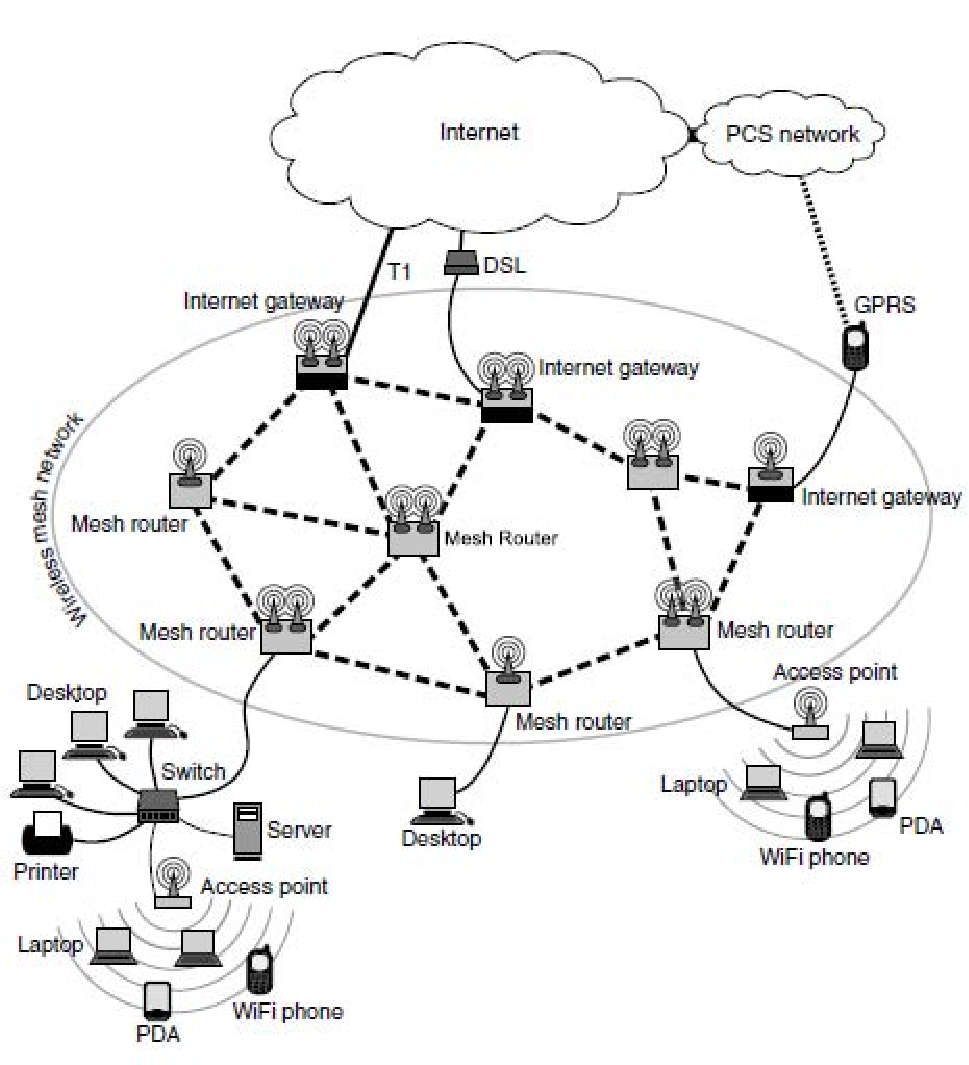
\includegraphics[width=.5\textwidth]{images/wmn_general}
    \caption{Wireless Mesh Network General Architecture Overview~\cite{book1}}
    \label{fig:wmn_general}
\end{figure}

if something referring to this figure, use this \ref{fig:wmn_general}


Testing; just making references show
asdf ~\cite{wearable}.
asdf ~\cite{adhocmsgferry}.
asdf ~\cite{hybrid}.
asdf ~\cite{QoSrouting}.
asdf ~\cite{efficientrouting}.
asdf ~\cite{implement}.
asdf ~\cite{book1}.


\chapter{Project Scenario \& Model Design} 

Any application running over a message ferrying network must have the following characteristics
\begin{description}
\item[Delay Tolerance: ]
Since data is transported by a physical device, significant delays of minutes to hours must be expected.
\item[Loss Tolerance: ]
Given that ferries have limited memory, loss of data must be expected.
\item[Loss Tolerance: ]
Given that ferries have limited memory, loss of data must be expected.
\item[Small and Independent Messages: ]
Following from the limited memory capacity of ferries and the high probability of packet loss, a reliable method for segmentation and reassembly messages should not be expected. 
Applications should limit the size of messages such that the can be transmitted in their entirety using one network packet.
(See section \ref{sec:fountain_codes} for future work)
\end{description}

Given these criteria, a message ferrying network is unsuitable for many classic networking applications such as web browsing, real-time voice or text communication and file transfer.
As such, a very specialized network designed for 

\chapter{Simulation}

%--------------------------------------------------------------------------------------------------------
% 		Intro
%--------------------------------------------------------------------------------------------------------
%\section{Intro}

This chapter provides an overview of the two simulations which were created.
%, we create realistic scenarios that model the environments of some of its applications.  
These simulations are intended to be as realistic as possible and involve random movement of ferry nodes.
The ferries were assumed to be vehicles which defined their speed.
A number of scenarios were tested for each simulation, the parameters varied are explained in section \ref{sec:metrics}.

%More realistic scenario
%	- Random ferry movement
%		- Details -> car
%	- even source spacing

%--------------------------------------------------------------------------------------------------------
% 		Topology
%--------------------------------------------------------------------------------------------------------
\section{Network Model}
\label{sec:main_net_model}

This section outlines the two network models defining each simulation. 
Their difference lies on the number of ferry and gateway nodes.
The parameters common between each are explained in section \ref{sec:commonsettings}.

\subsection{Scenario 1}		%1 gateway, 1 ferry

The first simulation was created with one gateway node, one ferry node, and ten source nodes.
The network model may be seen in figure \ref{fig:scenario2}.
The gateway is placed in the center of the map and the ferry node starts next to it.
Source nodes are more or less evenly distributed and are placed such that they are out of direct communication range.

%picture of the scenario2 (1f1g random movement)
\begin{figure}[ht]
    \centering
    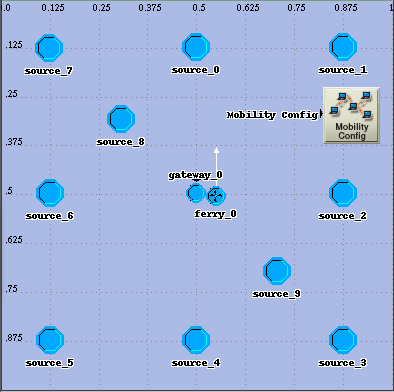
\includegraphics[width=0.6\textwidth]{images/scenario2-top}
    \caption{Simulation 1 - Network Model (1 Gateway, 1 Ferry)}
    \label{fig:scenario2}
\end{figure}

\subsection{Scenario 2}		%2 gateways, 2 ferries

The second simulation was created with two gateway nodes, two ferry node, and ten source nodes.
The network model may be seen in figure \ref{fig:scenario3}.
The gateways are placed in opposing quadrants, while both ferries start from the center.
Source nodes and gateways are more or less evenly distributed and are placed such that they are out of direct communication range.

\begin{figure}[ht]
    \centering
    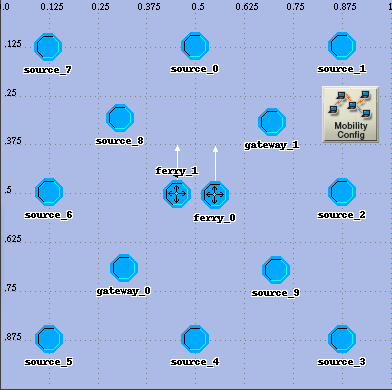
\includegraphics[width=0.6\textwidth]{images/scenario3-top}
    \caption{Simulation 2 - Network Model (2 Gateways, 2 Ferries)}
    \label{fig:scenario3}
\end{figure}

\subsection{Common Settings}
\label{sec:commonsettings}

Some of the settings and characteristics common to all the topologies are the following:
\begin{itemize}
	\item All ferries move in random directions and have a varying speeds of 36kph - 72kph in uniform distribution.
	\item The size of both maps is 1km x 1km
	%\item Beaconing intervals  %TO DO
	\item Properties are updated every 2 seconds with a variance of 0.1 seconds
	\item Simulations are run for 90 minutes. 
	Property updates were disabled for the last thirty minutes in an effort to obtain statistics valid for a simulation of indefinite length. 
\end{itemize}

%--------------------------------------------------------------------------------------------------------
% 		Metrics and Results of Interest 
%--------------------------------------------------------------------------------------------------------
\section{Metrics and Results of Interest }
\label{sec:metrics}

Two metrics are of primary interest when analyzing the network, update success rate and delay.

\subsection{Update Success Rate}
\label{sec:packetloss}

Update success rate, or alternatively update loss, is of central importance in the network.
It is primarily affected by memory limits imposed by the ferry but is also affected by the number of ferry and gateway nodes.
Defining success rate is somewhat complicated as updates may be intentionally discarded before they reach a gateway if they are out of date.
Additionally, updates may be duplicated multiple time as ferries exchange messages.
Finally, discarding updates with a key update number less than the most recent key update number received by the gateway is desired behaviour.
As such, the following conditions are used to determine success rate which is measured as \emph{success}, \emph{failure} or \emph{no value} for each key update generated by every source node property.

\begin{itemize}
\item For updates which reach the gateway:
	\begin{itemize}
	\item If the update has a key update number greater than the last update received by the gateway (for a given source id and property key) the update counts as a \emph{success}.
	\item If the update has a key update number equal to or less than the last update received by the gateway (for a given source id and property key) the update is not considered and counts as \emph{no value}.
	\end{itemize}
\item For updates which do not reach the gateway and are discard by every ferry node:
	\begin{itemize}
	\item If the update has a key update number greater than the last update received by the gateway (for a given source id and property key) the update counts as a \emph{failure}.
	\item If the update has a key update number equal to or less than the last update received by the gateway (for a given source id and property key) the update is not considered and counts as \emph{no value}.
	\end{itemize}
\end{itemize}

\subsection{Delay}
\label{sec:delay}

The number of ferries and gateways is the primary parameter affecting delay, however, ferry memory limits also play a role.
Delay is defined as the time an update takes to reach the gateway after it has been generated by a source node.
Only updates which are successfully delivered (as defined in section \ref{sec:packetloss}) 
count towards delay.
As such, it is important for results of delay to be considered within the context of update success rate.
It should be noted that the lower bound on delay is the time it physically takes the ferry to move between the source node and gateway.

\subsection{Simulation Parameters Varied} %TODO: better section title

The following parameters were varied to create additional scenarios for each simulation as presented in section \ref{sec:main_net_model}. 
Their impact on success rate and delay (from sections \ref{sec:delay} and \ref{sec:packetloss}) were considered.
  
\subsubsection{Memory Limit}
\label{sec:mainMemLimit}
The memory limit, also referred to as capacity, is the buffer size of the ferry.
It limits the number of unique updates which can be stored at once.
It is set in number of updates, not bytes, and hence is somewhat unrealistic.
It is sufficient for the purposes of this scenario however.

\subsubsection{Seed - Effect of Randomness}
Since ferry movement is random and the number of gateways is limited, it is important to consider multiple random when simulating in OPNET. 

%TODO: why important

\subsubsection{Source Node Storage}
\label{sec:source_node_storage}
The node models and algorithm presented thus far has assumed that only ferries store updates. 
A modified node model which allows source nodes to store updates was also considered.
The effect of enabling source node storage was examined.

%This is an option that allows the source nodes to be able to store update packets for the ferry nodes, which will then provide better ranges of transfer.


\chapter{Results}

\section{Success Rate}

\subsection{Simulation 1}

\begin{figure}[h!]
    \centering
    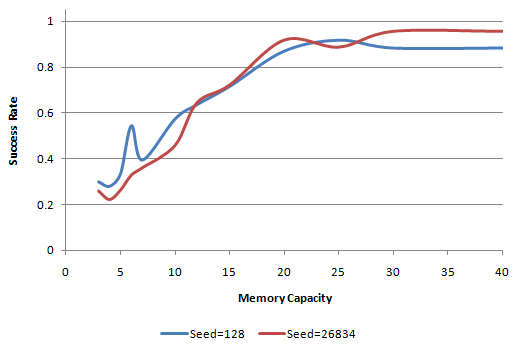
\includegraphics[width=.9\textwidth]{images/result_sccess_sim1byseed_dss}
    \caption{TODO}
    %\label{fig:moistureSensor}
\end{figure}

\subsection{Simulation 2}

\begin{figure}[h!]
    \centering
    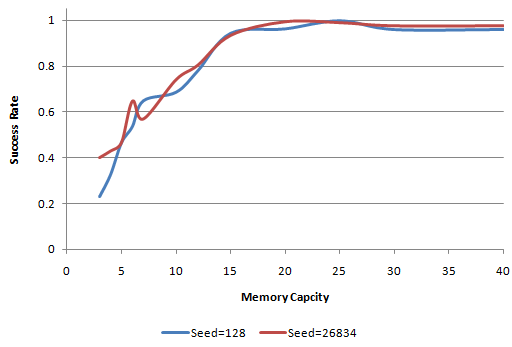
\includegraphics[width=.9\textwidth]{images/result_sccess_sim2byseed_dss}
    \caption{TODO}
    %\label{fig:moistureSensor}
\end{figure}

\subsection{Comparison of Success Rate}

\begin{figure}[h!]
    \centering
    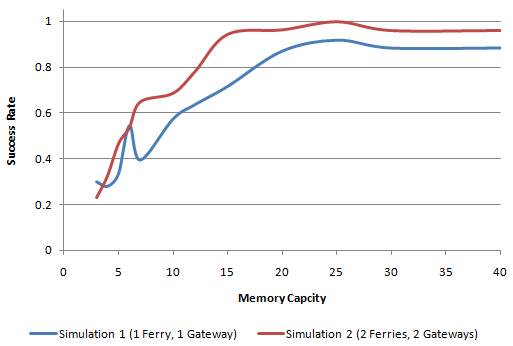
\includegraphics[width=.9\textwidth]{images/result_sccess_bothsim_128_dss}
    \caption{TODO}
    %\label{fig:moistureSensor}
\end{figure}

\subsection{Effect of Source Node Storage}

\begin{figure}[h!]
    \centering
    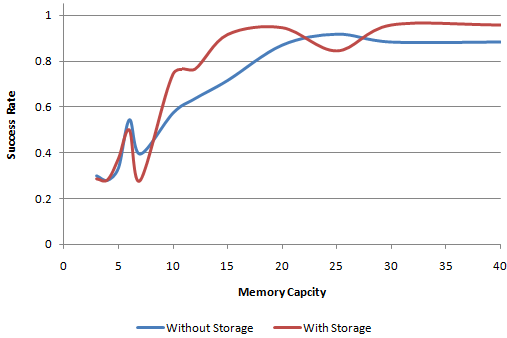
\includegraphics[width=.9\textwidth]{images/result_sccess_sim1byss_128}
    \caption{TODO}
    %\label{fig:moistureSensor}
\end{figure}


\begin{figure}[h!]
    \centering
    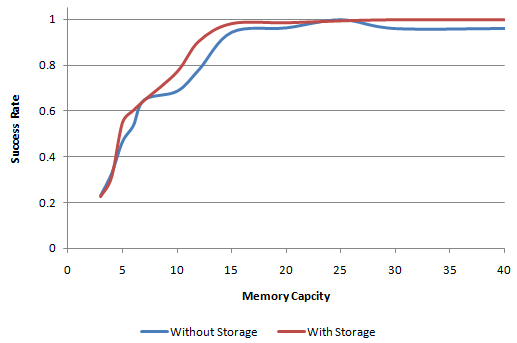
\includegraphics[width=.9\textwidth]{images/result_sccess_sim2byss_128}
    \caption{TODO}
    %\label{fig:moistureSensor}
\end{figure}

\section{Delay}

\chapter{Conclusion} 

First and foremost, OPNET has been shown to be a suitable tool for analyzing message ferrying.
The node models created to analyze the specialized \lq{}state monitor\rq{} network were tested and validated.
A more complicated examination was performed with a network model involving ten source nodes and varying numbers of ferry and gateway nodes.
Statistics measuring update success and delay were defined, implemented and collected during an OPNET simulation.

%TODO: Transition

\section{Results}

A number of general conclusions can be drawn from the results presented in \ref{sec:resultsChapter}.
Adding gateways and ferries was seen to reduces delay, reduces the memory requirements of ferries to achieve a desired success rate, and decreases variability in delay (see \ref{sec:results_success_s2}).
As such, any message ferrying network should have a maximum number of ferries and gateways.
Success rate was seen to marginally improve when enabling source storage.
This improvement is expected to increase with additional ferries.
As such, it may be concluded that networks with few ferries need not implement this feature, however it should enabled for networks with many ferries.

%NEED SOMETHING MORE

%An general discussion of results.
%Include a discussion on the feasibility of a practical implementation and what adoption threshold would be needed.

\section{Future Work}

There are four main categories for future work and improvements to the OPNET model in order to study task oriented message ferrying.

\subsection{Algorithm Improvements}

Many aspects of the ferrying algorithm implemented in this network are simplistic.
For example, there is no reverse communication from the gateway to message ferries indicating updates have been delivered and update messages may be discarded.
The implementation of an update acknowledgment mechanism could significantly improve performance and memory utilization.
Additionally, a more intelligent algorithm used by ferries to discard packets could also improve overall network performance.

\subsection{Model Improvements}

Many assumptions and simplifications were made when considering update and data transfer between nodes.
For example, near instantaneous data transfer, little to no packet loss, and a strict communication range of 60 meters was assumed.
Incorporating an existing point to point protocol for reliable wireless data transfer, such as WiFi or ZigBee would provide more realistic results.x

\subsection{Statistic Improvements}

Due to the unique nature of the network, common ways to measure statistics are not valid.
As such, custom logic was required to produce all statistics.
Measurement of only two statistics was implemented, delay and update success rate.
Adding additional statistics, such as number of active packets in the network and arrival order, would provide additional insights into the networks behaviour.

\subsection{Applicability and Network Model}

The simulation presented involves roughly even source node placement and random ferry movement.
It is unlikely that a real %change real
network would have these characteristics.
Creating and simulating a real-world network model and application would provide more realistic results.



%%%%%%%%%%%%%%%%%%%%%%%%%
% References
%%%%%%%%%%%%%%%%%%%%%%%%%

\bibliography{finalReport}
\addcontentsline{toc}{chapter}{\hspace{13pt}References}

%%%%%%%%%%%%%%%%%%%%%%%%%
% Appendix
%%%%%%%%%%%%%%%%%%%%%%%%%

\nothtml{
\begin{appendix}
%\appendix
%\renewcommand{\thechapter}{\Alph{chapter}}

\chapter{Code} 

%appendix A
%SOURCE KEY SINK MODEL

\section{Overview}
\begin{figure}[ht]
    \centering
    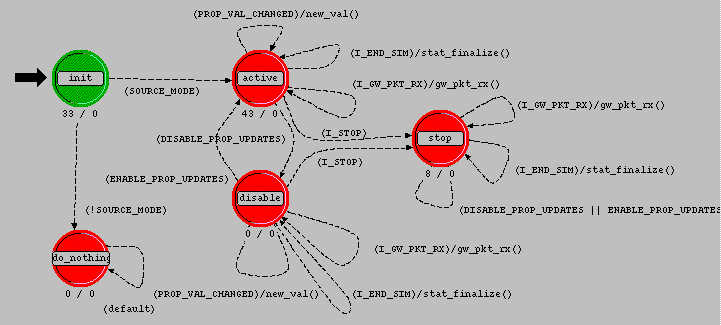
\includegraphics[scale=0.6]{images/p_source_property}
    \caption{Source property process model}
    \label{fig:appendix-a}
\end{figure}

\newpage

\section{Local variables}
\begin{figure}[ht]
    \centering
    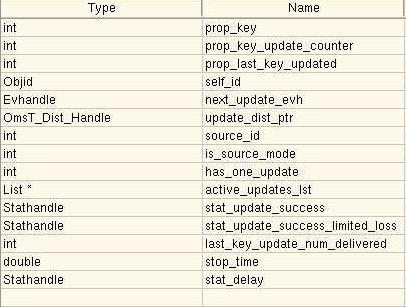
\includegraphics[width=.7\textwidth]{images/state_variable_source_property}
    \caption{State variables of source property process}
    \label{fig:appendix-a_sv}
\end{figure}

\section{Header Block}
%_____________________________________HEADER______________________________________
{\tiny
\begin{verbatim}
#include	<oms_dist_support.h>

//Interrupt Codes (codes have no meaning and are random)
#define IC_PROP_VAL_CHANGED 		39
#define IC_UPDATES_DISABLE	 		83
#define IC_UPDATES_ENABLE			84
#define IC_STOP					21
#define IC_GW_PKT_RX				99
#define SOURCE_MODE		(is_source_mode)

//Interrupts 
#define PROP_VAL_CHANGED	(op_intrpt_type() == OPC_INTRPT_SELF && op_intrpt_code() == IC_PROP_VAL_CHANGED)
#define DISABLE_PROP_UPDATES	(op_intrpt_type() == OPC_INTRPT_REMOTE && op_intrpt_code() == IC_UPDATES_DISABLE)
#define ENABLE_PROP_UPDATES	(op_intrpt_type() == OPC_INTRPT_REMOTE && op_intrpt_code() == IC_UPDATES_ENABLE)
#define I_GW_PKT_RX	(op_intrpt_type() == OPC_INTRPT_REMOTE && op_intrpt_code() == IC_GW_PKT_RX)
#define I_END_SIM	(op_intrpt_type() == OPC_INTRPT_ENDSIM)
#define I_STOP	(op_intrpt_type() == OPC_INTRPT_SELF && op_intrpt_code() == IC_STOP)

typedef struct
{
	int update_counter_number;
	int pkts_alive;
	int has_one_store;
	int gateway_rx;
	double generated_timestamp;
	int mark_for_delete;
	int discard_reason;
} active_update_tacker;

void new_val(void);
void schedule_update(void);
void gw_pkt_rx(void);
void stat_finalize(void);
\end{verbatim}
}

\section{Function Block}
%______________________________FUNCTION__________________________________
{\tiny
\begin{verbatim}

void new_val(void)
{
	FIN (new_val ());
	prop_key_update_counter++;
	schedule_update();
	FOUT
}
void schedule_update(void)
{
	double next_update_time;	
	FIN(schedule_update());
	next_update_time = oms_dist_outcome (update_dist_ptr);

	if (next_update_time <0)
	{
		next_update_time = 0;
	}

	next_update_evh      = op_intrpt_schedule_self (op_sim_time () + next_update_time, IC_PROP_VAL_CHANGED);
	FOUT;
}
void gw_pkt_rx()
{
	Ici *iciptr;
	int sourceid;
	int key_update_number;
	int action;
	int discard_reason;
	int tracker_index;
	double generated_timestamp;
	active_update_tacker *pTracker;
	char msg[255];
	int i;

	FIN(gw_pkt_rx());
	iciptr = op_intrpt_ici ();
	
	if(iciptr == OPC_NIL)
	{
		op_sim_end("Null ICI", "", "", "");
	}
	op_ici_attr_get (iciptr, "source_id", &sourceid);
	op_ici_attr_get (iciptr, "key_update_number", &key_update_number);
	op_ici_attr_get (iciptr, "action", &action);
	op_ici_attr_get (iciptr, "discard_reason", &discard_reason);
	op_ici_attr_get (iciptr, "generated_timestamp", &generated_timestamp);

	//Basic field checks 
	if(sourceid != source_id)
	{
		op_sim_end("Bad source id for ICI", "", "", "");
	}
	else if(key_update_number > prop_key_update_counter || key_update_number <= 0)
	{
		op_sim_end("Bad key_update_number for ICI", "", "", "");
	}	
	//Find the tracker
	pTracker = OPC_NIL;
	for(tracker_index = 0; tracker_index < op_prg_list_size(active_updates_lst); tracker_index++)
	{
		active_update_tacker *pTrackerTemp;
		pTrackerTemp = (active_update_tacker *)op_prg_list_access(active_updates_lst, tracker_index);
		
		if(pTrackerTemp->update_counter_number == key_update_number)
		{
			pTracker = pTrackerTemp;
			break;
		}
	}
	if(pTracker == OPC_NIL)
	{
		int i;
		char msg1[255];
		char msg2[255];
		char msg3[255];
		printf("Current list state\n");
		
		for(i = 0; i < op_prg_list_size(active_updates_lst); i++)
		{
			active_update_tacker *pTrackerTemp;
			pTrackerTemp = (active_update_tacker *)op_prg_list_access(active_updates_lst, i);	
			sprintf(msg1, "update_counter_number=%d\n", pTrackerTemp->update_counter_number);
			printf(msg1);
		}
		sprintf(msg1, "Tracker index=%d, List size=%d", tracker_index, op_prg_list_size(active_updates_lst));
		sprintf(msg2, "key_update_number=%d, prop_key_update_counter=%d", key_update_number, prop_key_update_counter);
		sprintf(msg3, "Action=%d", action);	
		op_sim_end("Could not find tracker", msg1, msg2, msg3);
	}
	if(action == 1)
	{
		//Gateway received packet
		if(pTracker->gateway_rx)
		{
			op_sim_end("Two gateway rx interrupts", "", "", "");
		}
		else if(pTracker->pkts_alive <= 0)
		{
			op_sim_end("pkts_alive problem", "", "", "");
		}
		pTracker->gateway_rx = 1;	
		op_stat_write(stat_delay, op_sim_time() - generated_timestamp);
		op_stat_write(stat_update_success, 1.0);
		op_stat_write(stat_update_success_limited_loss, 1.0);
		
		if(last_key_update_num_delivered >= key_update_number)
		{
			op_sim_end("Problem with gateway", "", "", "");
		}
		last_key_update_num_delivered = key_update_number;
	}
	else if (action == 2)
	{
		//Store	
		if(pTracker->pkts_alive < 0)
		{
			op_sim_end("Thats strange...", "", "", "");
		}	
		pTracker->pkts_alive++;
		pTracker->has_one_store = 1;
	}
	else if (action == 3)
	{
		//Discard
		pTracker->pkts_alive--;
		pTracker->discard_reason = discard_reason;
	}
	else
	{
		op_sim_end("Bad action", "", "", "");
	}
	has_one_update = 1;
	
	for(i = 0; i < op_prg_list_size(active_updates_lst); i++)
	{
		pTracker = (active_update_tacker *)op_prg_list_access(active_updates_lst, i);
	
		if(pTracker->pkts_alive <= 0)
		{
			pTracker->mark_for_delete--;
		}
		if(pTracker->mark_for_delete <= 0)
		{
			active_update_tacker *pTrackerTemp;
			
			if(pTracker->pkts_alive < 0 &&  pTracker->has_one_store)
			{
				op_sim_end("Thats strange...", "2", "", "");
			}	
			if(pTracker->gateway_rx == 0)
			{
				//Nothing left - update has been lost
				op_stat_write(stat_update_success, 0.0);
			
				if(pTracker->discard_reason == 1)
				{
					//Update
				}
				else if(pTracker->discard_reason == 2)
				{
					//Mem full
					if(pTracker->update_counter_number > last_key_update_num_delivered)
					{
						op_stat_write(stat_update_success_limited_loss, 0.0);
					}
				}
				else
				{
					op_sim_end("Bad discard reason", "", "", "");
				}
			}	
			pTrackerTemp = (active_update_tacker *)op_prg_list_remove(active_updates_lst, i);
			
			if(pTrackerTemp != pTracker)
			{
				op_sim_end("AHA,not another error!", "", "", "");
			}
			op_prg_mem_free(pTracker);
		}
	}
	op_ici_destroy(iciptr);
	FOUT;
}
void stat_finalize()
{
	Stathandle oneup;
	int i;

	FIN(stat_finalize());	
	oneup = op_stat_reg("One Update",OPC_STAT_INDEX_NONE, OPC_STAT_GLOBAL);	
	op_stat_write(oneup, has_one_update);
	
	for(i = 0; i < op_prg_list_size(active_updates_lst); i++)
	{
		active_update_tacker *pTracker;
		pTracker = (active_update_tacker *)op_prg_list_access(active_updates_lst, i);
		
		if(pTracker->gateway_rx == 0)
		{
			//Receiving should already have been taken care of
			op_stat_write(stat_update_success, 0.0);
			
			if(pTracker->update_counter_number > last_key_update_num_delivered)
			{
				op_stat_write(stat_update_success_limited_loss, 0.0);
			}
		}
		
		if(pTracker->update_counter_number == prop_last_key_updated)
		{
			if(pTracker->gateway_rx == 0)
			{
				op_stat_write(stat_delay, op_sim_time() - pTracker->generated_timestamp);
			}
		}
	}
	FOUT;
}
\end{verbatim}
}
\section{init State: Enter Executives}
%______________________________________Init_____________________________________________________________
{\tiny
\begin{verbatim}
char msg[100];
char updatedist_str [128];
self_id = op_id_self();
op_ima_obj_attr_get (self_id, "Source ID", &source_id);
op_ima_obj_attr_get (self_id, "Property Key", &prop_key);
op_ima_obj_attr_get (self_id, "Property Update Interval", updatedist_str);
op_ima_obj_attr_get (self_id, "Stop Time", &stop_time);
op_ima_obj_attr_get (self_id, "Enable Properties", &is_source_mode);
active_updates_lst = op_prg_list_create();
has_one_update = 0;
prop_key_update_counter = 0;
prop_last_key_updated = 0; //So it gets updated right away
update_dist_ptr = oms_dist_load_from_string (updatedist_str);
stat_delay = op_stat_reg("Delay",OPC_STAT_INDEX_NONE, OPC_STAT_GLOBAL);
stat_update_success = op_stat_reg("Update Success",OPC_STAT_INDEX_NONE, OPC_STAT_GLOBAL);
stat_update_success_limited_loss = op_stat_reg("Update Success - Losses by buffer full",OPC_STAT_INDEX_NONE, OPC_STAT_GLOBAL);

if(is_source_mode)
{
	schedule_update();	
	if(stop_time > 0)
	{
		op_intrpt_schedule_self (op_sim_time() + stop_time, IC_STOP);
	}
}
\end{verbatim}
}

\section{active State: Enter Executives}
%______________________________________Active_____________________________________________________________
{\tiny
\begin{verbatim}
Packet *pPkt;
if(prop_key_update_counter != prop_last_key_updated)
{
	active_update_tacker *pTracker;
	int i;
	
	//Error check
	for(i = 0; i < op_prg_list_size(active_updates_lst); i++)
	{
		//Might be able to just check the tail instead
	
		pTracker = (active_update_tacker *)op_prg_list_access(active_updates_lst, i);
		if(pTracker->update_counter_number == prop_last_key_updated)
		{
			if(pTracker->has_one_store == 0)
			{
				op_sim_end("Did not receive store interrupt", "", "", "");
			}
		}
	}
	prop_last_key_updated = prop_key_update_counter;
	pPkt = op_pk_create_fmt("keyupdate");
	op_pk_nfd_set_int32(pPkt, "source_id", source_id);		
	op_pk_nfd_set_int32(pPkt, "key", prop_key);	
	op_pk_nfd_set_int32(pPkt, "key_update_number", prop_key_update_counter);
	op_pk_nfd_set_dbl(pPkt, "generated_timestamp", op_sim_time());
	op_pk_nfd_set_objid(pPkt, "source_prop_objid", self_id);
	pTracker = (active_update_tacker *) op_prg_mem_alloc (sizeof (active_update_tacker));
	pTracker->update_counter_number = prop_key_update_counter;
	pTracker->pkts_alive = 0;
	pTracker->has_one_store = 0;
	pTracker->gateway_rx = 0;
	pTracker->generated_timestamp = op_sim_time();
	pTracker->mark_for_delete = 3;
	op_prg_list_insert(active_updates_lst, pTracker, OPC_LISTPOS_TAIL);	
	op_pk_send(pPkt, 0); //Output stream
}
\end{verbatim}
}

\section{stop State: Enter Executives}
%_____________________________________Stop_____________________________________________________________
{\tiny
\begin{verbatim}
char msg_str[255];
if (op_ev_valid (next_update_evh) == OPC_TRUE)
{
	sprintf(msg_str, "[%d] Stopping property updates @ %d\n", source_id, op_sim_time());
	printf(msg_str);
	op_ev_cancel (next_update_evh);
}
\end{verbatim}
}	%source property

\cleardoublepage

%appendix B
%p_storage

\section{Process: Storage}

\subsection{Visual}
\begin{figure}[ht]
    \centering
    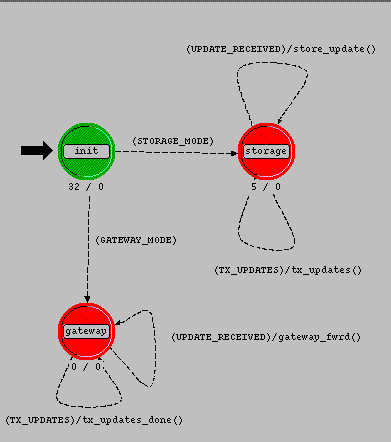
\includegraphics[scale=0.5]{images/p_storage}
    \caption{Storage process model}
    \label{fig:appendix-b}
\end{figure}

\subsection{Local variables}
\begin{figure}[h]
    \centering
    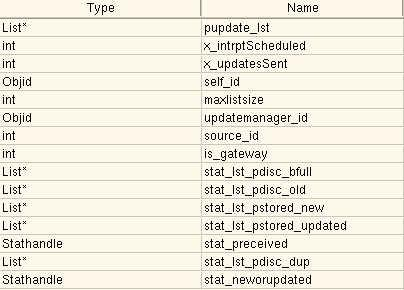
\includegraphics[width=.7\textwidth]{images/state_variable_storage}
    \caption{State variables of storage process}
    \label{fig:appendix-b_sv}
\end{figure}

\subsection{Header Block}
%_____________________________________HEADER______________________________________
{\tiny
\begin{verbatim}
#define MAX_SRC_IDS		10
#define GATEWAY_MODE	(is_gateway)
#define STORAGE_MODE	(!GATEWAY_MODE)
#define STRM_UM_IN		0
#define STRM_UM_OUT		0
#define STRM_GW_OUT		1
//Interrupt Codes (random numbers)
#define IC_DUMP_UPDATES 		73
#define IC_DUMP_UPDATES_DONE 	74
#define IC_SOURCPROP_ACTION 99
#define TX_UPDATES 		(op_intrpt_type() == OPC_INTRPT_REMOTE && op_intrpt_code() == IC_DUMP_UPDATES)
#define UPDATE_RECEIVED	(op_intrpt_type() == OPC_INTRPT_STRM)

int written_global_storage_stat = 0;
List *create_stat_lst_loc(const char *);
void store_update(void);
void tx_updates(void);
void gateway_fwrd(void);
\end{verbatim}
}

\subsection{Function Block}
%______________________________FUNCTION__________________________________
{\tiny
\begin{verbatim}
void store_update(void)
{
	Packet *pkt;
	Packet *lstPkt;
	char message_str [255];
	Objid prop1_id;
	int key;
	int sourceid;
	int key_updnm;
	int pos_index;
	double gen_ts;
	int newkey;
	int newsourceid;
	int newkey_updnm;
	double newgen_ts;
	int listsize;
	int i, j, k;
	double temp;
	Ici *iciptr;
	Objid source_prop_id;	
	FIN (store_update ());
	pkt = op_pk_get (op_intrpt_strm ());
	
	//get info
	op_pk_nfd_get(pkt, "key", &newkey);
	op_pk_nfd_get(pkt, "source_id", &newsourceid);
	op_pk_nfd_get(pkt, "key_update_number", &newkey_updnm);
	op_pk_nfd_get(pkt, "generated_timestamp", &newgen_ts);
	listsize = op_prg_list_size(pupdate_lst);
	
	if(newsourceid < 0 || newsourceid >= MAX_SRC_IDS)
	{
		op_sim_end("Bad sourceid", "", "", "");
	}
	op_stat_write(stat_preceived, 1.0);
	
	//Search & Compare 'key_update_number'; replace if newer
	for(i = 0; i < listsize; i++)
	{
		lstPkt = (Packet *)op_prg_list_access (pupdate_lst, i);
		op_pk_nfd_get(lstPkt, "key", &key);
		op_pk_nfd_get(lstPkt, "source_id", &sourceid);
		op_pk_nfd_get(lstPkt, "key_update_number", &key_updnm);
		op_pk_nfd_get(lstPkt, "generated_timestamp", &gen_ts);
	
		//COMPARE for matching source/key
		if(newsourceid == sourceid)
		{
			if(newkey == key)
			{
				if(newkey_updnm > key_updnm)	//if key is newer we update
				{
					if(newsourceid != source_id)
					{
						op_stat_write(*((Stathandle *)op_prg_list_access (stat_lst_pstored_updated, sourceid)), 1.0);
						op_stat_write(stat_neworupdated, 1.0);
					}
					op_pk_nfd_get(lstPkt, "source_prop_objid", &source_prop_id);
					iciptr = op_ici_create ("prop_action");
					op_ici_attr_set (iciptr, "source_id", sourceid);
					op_ici_attr_set (iciptr, "key_update_number", newkey_updnm);
					op_ici_attr_set (iciptr, "action", 2);
					op_ici_install(iciptr);
					op_intrpt_schedule_remote (op_sim_time (), IC_SOURCPROP_ACTION, source_prop_id);

					iciptr = op_ici_create ("prop_action");
					op_ici_attr_set (iciptr, "source_id", sourceid);
					op_ici_attr_set (iciptr, "key_update_number", key_updnm);
					op_ici_attr_set (iciptr, "action", 3); //3 = discard
					op_ici_attr_set (iciptr, "discard_reason", 1); //1 = update
					op_ici_install(iciptr);
					op_intrpt_schedule_remote (op_sim_time (), IC_SOURCPROP_ACTION, source_prop_id);
										
					op_prg_list_remove (pupdate_lst, i);
					op_prg_list_insert(pupdate_lst, pkt, OPC_LISTPOS_TAIL);
					op_pk_destroy(lstPkt);
					FOUT;
				}
				else
				{
					if(newkey_updnm == key_updnm)
					{
						op_stat_write(*((Stathandle *)op_prg_list_access (stat_lst_pdisc_dup, sourceid)), 1.0);
					}
					else
					{
						op_stat_write(*((Stathandle *)op_prg_list_access (stat_lst_pdisc_old, sourceid)), 1.0);
					}
					//Dont need to trigger the source prop intrupt because this pkt was never stored
					op_pk_destroy(pkt);
					FOUT;
				}
			}
		}
	} //forloop

	op_pk_nfd_get(pkt, "source_prop_objid", &source_prop_id);				
	iciptr = op_ici_create ("prop_action");
	op_ici_attr_set (iciptr, "source_id", newsourceid);
	op_ici_attr_set (iciptr, "key_update_number", newkey_updnm);
	op_ici_attr_set (iciptr, "action", 2); //2 = store
	op_ici_install(iciptr);
	op_intrpt_schedule_remote (op_sim_time (), IC_SOURCPROP_ACTION, source_prop_id);
	op_prg_list_insert(pupdate_lst, pkt, OPC_LISTPOS_TAIL);
	listsize = op_prg_list_size(pupdate_lst);

	if(newsourceid != source_id)
	{
		op_stat_write(*((Stathandle *)op_prg_list_access (stat_lst_pstored_new, newsourceid)), 1.0);
		op_stat_write(stat_neworupdated, 1.0);
	}
	//See if we need to get rid of something
	if(listsize > maxlistsize)
	{	
		//set first packet for temp
		lstPkt = (Packet *)op_prg_list_access (pupdate_lst, 0);
		op_pk_nfd_get(lstPkt, "generated_timestamp", &gen_ts);
		temp = gen_ts;
		
		//find oldest timestamp
		for(j = 0; j < listsize; j++)
		{
			lstPkt = (Packet *)op_prg_list_access (pupdate_lst, j);
			op_pk_nfd_get(lstPkt, "generated_timestamp", &gen_ts);		
			if(gen_ts < temp)
			{
				temp = gen_ts;	//replace if older
			}
		}
	
		//delete packet with oldest timestamp, temp, 
		for(k = 0; k < listsize; k++)
		{
			lstPkt = (Packet *)op_prg_list_access (pupdate_lst, k);
			op_pk_nfd_get(lstPkt, "generated_timestamp", &gen_ts);
			op_pk_nfd_get(lstPkt, "source_id", &sourceid);
			op_pk_nfd_get(lstPkt, "key_update_number", &key_updnm);
			
			if(temp == gen_ts)
			{
				op_stat_write(*((Stathandle *)op_prg_list_access (stat_lst_pdisc_bfull, sourceid)), 1.0);
				op_pk_nfd_get(lstPkt, "source_prop_objid", &source_prop_id);				
				iciptr = op_ici_create ("prop_action");
				op_ici_attr_set (iciptr, "source_id", sourceid);
				op_ici_attr_set (iciptr, "key_update_number", key_updnm);
				op_ici_attr_set (iciptr, "action", 3); //3 = discard
				op_ici_attr_set (iciptr, "discard_reason", 2); //2 = Memory Full
				op_ici_install(iciptr);
				op_intrpt_schedule_remote (op_sim_time (), IC_SOURCPROP_ACTION, source_prop_id);				
				op_prg_list_remove (pupdate_lst, k);
				op_pk_destroy(lstPkt);

				break;
			}
		}
	}
	FOUT;
}
void tx_updates(void)
{
	int i;
	int lstSize;
	Packet *pkt;
	Packet *pPktCopy;
	char message_str [255];	
	FIN (tx_updates ());
	
	lstSize = op_prg_list_size (pupdate_lst);
	for (i = 0; i < lstSize; i++)
	{
		pkt = (Packet *) op_prg_list_access (pupdate_lst, i);		
		pPktCopy = op_pk_copy(pkt);
		op_pk_send(pPktCopy, STRM_UM_OUT);
	}
	op_intrpt_schedule_remote(op_sim_time(), IC_DUMP_UPDATES_DONE, updatemanager_id);
	FOUT;
}
void tx_updates_done(void)
{
	FIN (tx_updates_done ());	
	op_intrpt_schedule_remote(op_sim_time(), IC_DUMP_UPDATES_DONE, updatemanager_id);
	FOUT;
}
void gateway_fwrd()
{
	FIN (update_gateway ());
	op_stat_write(stat_preceived, 1.0);
	op_pk_send(op_pk_get(STRM_UM_IN), STRM_GW_OUT);
	FOUT;
}
List *create_stat_lst_loc(const char *statName)
{
	List *lst;
	int stat_size_asdf;
	int i;
	char msg1[255];
	char msg2[255];
	
	FIN(create_stat_lst_loc());	
	op_stat_dim_size_get(statName, OPC_STAT_LOCAL, &stat_size_asdf);
	if(stat_size_asdf != MAX_SRC_IDS)
	{
		sprintf(msg1, "stat_size_asdf: %d", stat_size_asdf);
		sprintf(msg2, "MAX_SRC_IDS: %d", MAX_SRC_IDS);
		op_sim_end("Bad stat dimension", statName, msg1, msg2);
	}
	lst = op_prg_list_create();
	for(i = 0; i < MAX_SRC_IDS; i++)
	{
		Stathandle *sth_temp;
		sth_temp = (Stathandle *) op_prg_mem_alloc (sizeof (Stathandle));
		*sth_temp = op_stat_reg (statName, i, OPC_STAT_LOCAL);
		
		op_prg_list_insert(lst, sth_temp, OPC_LISTPOS_TAIL);
	}
	FRET(lst);
}
\end{verbatim}
}
\subsection{Init State}
%______________________________________Init_____________________________________________________________
{\tiny
\begin{verbatim}
int i;
self_id = op_id_self();
printf("REGISTERING STATS\n");
stat_lst_pstored_new = create_stat_lst_loc("Pkts Stored - New");
stat_lst_pstored_updated = create_stat_lst_loc("Pkts Stored - Updated");
stat_lst_pdisc_old = create_stat_lst_loc("Pkts Discarded - Old");
stat_lst_pdisc_bfull = create_stat_lst_loc("Pkts Discarded - Buffer Full");
stat_lst_pdisc_dup = create_stat_lst_loc("Pkts Discarded - Duplicate");
stat_preceived = op_stat_reg("Pkts Received",OPC_STAT_INDEX_NONE, OPC_STAT_LOCAL);
stat_neworupdated = op_stat_reg("Pkts Stored - New or Updated",OPC_STAT_INDEX_NONE, OPC_STAT_LOCAL);

pupdate_lst = op_prg_list_create (); 		//allocate an empty list
op_ima_sim_attr_get (OPC_IMA_INTEGER, "Capacity", &maxlistsize);
if(written_global_storage_stat == 0)
{
	written_global_storage_stat = 1;
	op_stat_write_scalar("Storage Capacity", maxlistsize);
}
op_ima_obj_attr_get (self_id, "Source ID", &source_id);
op_ima_obj_attr_get (self_id, "Is Gateway", &is_gateway);
updatemanager_id = op_id_from_name (op_topo_parent(self_id), OPC_OBJTYPE_PROC, "update_manager");
\end{verbatim}
}

\subsection{Storage State}
%______________________________________Storage_____________________________________________________________
{\tiny
\begin{verbatim}
if(maxlistsize <= 0)
{
	//Typically when this node is a gateway
	op_sim_end("Invalid max list size", "", "", "");
}
\end{verbatim}
}
	%storage

\cleardoublepage

%%appendix E
%Update Manager

\section{Overview}
\begin{figure}[ht]
    \centering
    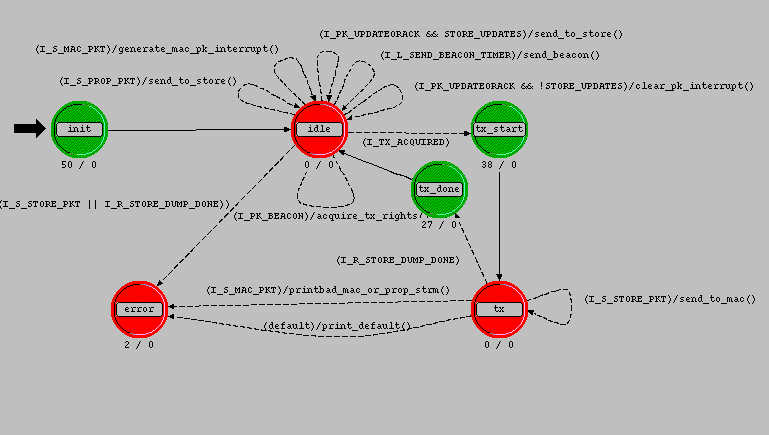
\includegraphics[scale=0.6]{images/p_update_manager}
    \caption{Update manager process model}
    \label{fig:appendix-c}
\end{figure}

\newpage

\section{Local variables}
\begin{figure}[ht]
    \centering
    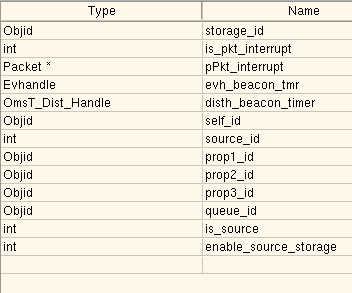
\includegraphics[width=.7\textwidth]{images/state_variable_update_manager}
    \caption{State variables of update manager process}
    \label{fig:appendix-c_sv}
\end{figure}

\section{Header Block}
%_____________________________________HEADER______________________________________
{\tiny
\begin{verbatim}

#include	<oms_dist_support.h>
//STREAMS
#define STRM_IN_P1		0
#define STRM_IN_P2		1
#define STRM_IN_P3		2
#define STRM_IN_STORE	3
#define STRM_OUT_STORE	0
#define STRM_IN_MAC	4
#define STRM_OUT_MAC 	1

//INTERRUPT CODES
#define IC_REQ_STORE_DUMP		73
#define IC_STORE_DUMP_DONE		74
#define IC_PROP_UPDATES_DISABLE	83
#define IC_PROP_UPDATES_ENABLE		84
#define IC_SEND_BEACON_TIMER		42
#define IC_PK_UPDATEORACK		37
#define IC_PK_BEACON			38
#define IC_Q_DISABLE			54
#define IC_Q_ENABLE			55
#define IC_TX_ACQUIRED			67

//INTERRUPTS

//Stream
#define I_S_PROP_PKT	(op_intrpt_type() == OPC_INTRPT_STRM && (op_intrpt_strm() == STRM_IN_P1 || op_intrpt_strm() == STRM_IN_P2 || op_intrpt_strm() == STRM_IN_P3))
#define I_S_STORE_PKT	(op_intrpt_type() == OPC_INTRPT_STRM && op_intrpt_strm() == STRM_IN_STORE)
#define I_S_MAC_PKT	(op_intrpt_type() == OPC_INTRPT_STRM && op_intrpt_strm() == STRM_IN_MAC)

//Packet op_intrpt_strm() == STRM_IN_P1
#define I_PK_UPDATEORACK	(op_intrpt_type() == OPC_INTRPT_SELF && op_intrpt_code() == IC_PK_UPDATEORACK)
#define I_PK_BEACON	(op_intrpt_type() == OPC_INTRPT_SELF && op_intrpt_code() == IC_PK_BEACON)
#define I_TX_ACQUIRED	((op_intrpt_type() == OPC_INTRPT_SELF || op_intrpt_type() == OPC_INTRPT_REMOTE) && op_intrpt_code() == IC_TX_ACQUIRED)

//Remote
#define I_R_STORE_DUMP_DONE	(op_intrpt_type() == OPC_INTRPT_REMOTE && op_intrpt_code() == IC_STORE_DUMP_DONE)

//Local (self)
#define I_L_SEND_BEACON_TIMER 	(op_intrpt_type() == OPC_INTRPT_SELF && op_intrpt_code() == IC_SEND_BEACON_TIMER)

//OTHER
#define STORE_UPDATES			(!is_source || enable_source_storage)
List *tx_rights_lst = OPC_NIL;

//PROTOTYPES

//Beacon control
void enable_beacon();
void disable_beacon();
void send_beacon();
void send_beacon_timed();
void reset_beacon_timer();
//Property control
void enable_prop_updates();
void disable_prop_updates();
void disable_q();
void enable_q();
//Storage control
void request_storage_dump();
//Packet redirection 
void send_to_store();
void send_to_mac();
void generate_mac_pk_interrupt();
void clear_pk_interrupt(void);
void printbad_mac_or_prop_strm(void);
void print_default(void);
void acquire_tx_rights(void);

\end{verbatim}
}

\section{Function Block}
%______________________________FUNCTION__________________________________
{\tiny
\begin{verbatim}

void schedule_beacon()
{
	double next_becon_time = 0;
	FIN(schedule_beacon());
	while(next_becon_time <= 0.1)
	{
		next_becon_time = oms_dist_outcome (disth_beacon_timer);
	}
	evh_beacon_tmr = op_intrpt_schedule_self (op_sim_time () + next_becon_time, IC_SEND_BEACON_TIMER);
	FOUT;
}
void enable_beacon()
{
	FIN(enable_beacon());
	schedule_beacon();
	FOUT;
}
void disable_beacon()
{
	FIN(disable_beacon());
	if (op_ev_valid (evh_beacon_tmr) == OPC_TRUE)
	{
		op_ev_cancel (evh_beacon_tmr);
	}
	FOUT;
}
void reset_beacon_timer()
{
	FIN(reset_beacon_timer());
	disable_beacon();
	enable_beacon();
	FOUT;
}
void send_beacon()
{
	char message_str[255];
	Packet *pPkt;
	FIN(send_beacon());
	pPkt = op_pk_create_fmt("beacon");
	op_pk_nfd_set_int32(pPkt, "source_id", source_id);
	op_pk_send(pPkt, STRM_OUT_MAC);
	schedule_beacon();
	FOUT;
}
//Property control
void enable_prop_updates()
{
	FIN(enable_prop_updates());
	op_intrpt_schedule_remote(op_sim_time(), IC_PROP_UPDATES_ENABLE, prop1_id);
	op_intrpt_schedule_remote(op_sim_time(), IC_PROP_UPDATES_ENABLE, prop2_id);
	op_intrpt_schedule_remote(op_sim_time(), IC_PROP_UPDATES_ENABLE, prop3_id);
	FOUT;
}
void disable_prop_updates()
{
	FIN(disable_prop_updates());
	op_intrpt_schedule_remote(op_sim_time(), IC_PROP_UPDATES_DISABLE, prop1_id);
	op_intrpt_schedule_remote(op_sim_time(), IC_PROP_UPDATES_DISABLE, prop2_id);
	op_intrpt_schedule_remote(op_sim_time(), IC_PROP_UPDATES_DISABLE, prop3_id);
	FOUT;
}
void request_storage_dump()
{
	FIN(request_sotrage_dump());
	op_intrpt_schedule_remote(op_sim_time(), IC_REQ_STORE_DUMP, storage_id);
	FOUT;
}
void send_to_store()
{
	Packet *pPktToForward;
	FIN(send_to_store());
	if(is_pkt_interrupt)
	{
		is_pkt_interrupt = 0;
		if(pPkt_interrupt == OPC_NIL)
		{
			op_sim_end("Nill interrupt pkt", "", "", "");	
		}
		pPktToForward = pPkt_interrupt;
		pPkt_interrupt = OPC_NIL;
	}
	else
	{
		if(pPkt_interrupt != OPC_NIL)
		{
			op_sim_end("Not nill interrupt pkt", "", "", "");	
		}
		pPktToForward = op_pk_get(op_intrpt_strm());
	}
	op_pk_send(pPktToForward, STRM_OUT_STORE);
	FOUT;
}
void send_to_mac()
{
	char message_str[255];
	Packet *pPktToForward;
	FIN(send_to_mac());
	if(is_pkt_interrupt)
	{
		is_pkt_interrupt = 0;
		if(pPkt_interrupt == OPC_NIL)
		{
			op_sim_end("Nill interrupt pkt", "", "", "");	
		}
		pPktToForward = pPkt_interrupt;
		pPkt_interrupt = OPC_NIL;
	}
	else
	{
		if(pPkt_interrupt != OPC_NIL)
		{
			op_sim_end("Not nill interrupt pkt", "", "", "");	
		}
		pPktToForward = op_pk_get(op_intrpt_strm());
	}
	op_pk_send(pPktToForward, STRM_OUT_MAC);
	FOUT;
}
void clear_pk_interrupt()
{
	FIN(clear_pk_interrupt());
	if(is_pkt_interrupt)
	{
		is_pkt_interrupt = 0;
		if(pPkt_interrupt == OPC_NIL)
		{
			op_sim_end("Nill interrupt pkt", "", "", "");	
		}
		op_pk_destroy(pPkt_interrupt);
		pPkt_interrupt = OPC_NIL;
	}
	else
	{
		op_sim_end("clear_pk_interrupt called wrong", "", "", "");	
	}
	FOUT;
}
void generate_mac_pk_interrupt()
{
	char message_str[255];
	char format_name[255];
	FIN(generate_mac_pk_interrupt());
	reset_beacon_timer(); //To prevent a bad state
	if(pPkt_interrupt != OPC_NIL)
	{
		op_sim_end("Not nill interrupt pkt", "", "", "");	
	}
	else if (is_pkt_interrupt)
	{
		op_sim_end("Pkt interrupt flag set (bad)", "", "", "");		
	}
	else if(op_intrpt_strm() != STRM_IN_MAC)
	{
		op_sim_end("generate_mac_pk_interrupt called for non mac stream interrupt", "", "", "");	
	}
	pPkt_interrupt = op_pk_get(STRM_IN_MAC);
	is_pkt_interrupt = 1;
	op_pk_format (pPkt_interrupt, format_name);
	if (strcmp (format_name, "beacon") == 0)
	{
		op_intrpt_schedule_self(op_sim_time(), IC_PK_BEACON);	
	}
	else if (strcmp (format_name, "keyupdate") == 0)
	{
		op_intrpt_schedule_self(op_sim_time(), IC_PK_UPDATEORACK);	
	}
	
	FOUT;
}
void disable_q()
{
	FIN(disable_q());
	op_intrpt_schedule_remote(op_sim_time(), IC_Q_DISABLE, queue_id);	
	FOUT;
}
void enable_q()
{
	FIN(enable_q());
	op_intrpt_schedule_remote(op_sim_time(), IC_Q_ENABLE, queue_id);	
	FOUT;
}
void print_default()
{
	FIN(print_default());
	printf("DEFAULT\n");
	FOUT;
}
void acquire_tx_rights()
{
	int i;
	FIN(acquire_tx_rights());
	if(is_pkt_interrupt)
	{
		is_pkt_interrupt = 0;
		
		if(pPkt_interrupt == OPC_NIL)
		{
			op_sim_end("Nill interrupt pkt", "", "", "");	
		}
		op_pk_destroy(pPkt_interrupt);
		pPkt_interrupt = OPC_NIL;
	}
	else
	{
		if(pPkt_interrupt != OPC_NIL)
		{
			op_sim_end("Not nill interrupt pkt", "", "", "");	
		}
	}
	for(i = 0; i < op_prg_list_size(tx_rights_lst); i++)
	{
		if(op_prg_list_access(tx_rights_lst, i) == &self_id)
		{
			if(i = 0)
			{
				op_sim_end("NOOOOO.......", "", "", "");	
			}
			FOUT;
		}
	}
	op_prg_list_insert(tx_rights_lst, &self_id, OPC_LISTPOS_TAIL);
	if(op_prg_list_size(tx_rights_lst) == 1)
	{
		op_intrpt_schedule_self(op_sim_time(), IC_TX_ACQUIRED);
	}
	FOUT;
}

\end{verbatim}
}

\section{init State: Enter Executives}
%______________________________________Init_____________________________________________________________
{\tiny
\begin{verbatim}


char beacon_dist_str[128];
self_id = op_id_self();
op_ima_obj_attr_get (self_id, "Source ID", &source_id);
op_ima_obj_attr_get (self_id, "Beacon Interval", beacon_dist_str);
disth_beacon_timer = oms_dist_load_from_string (beacon_dist_str);
op_ima_obj_attr_get (self_id, "Is Source", &is_source);
op_ima_sim_attr_get (OPC_IMA_INTEGER, "Enable Source Storage", &enable_source_storage);
storage_id = op_id_from_name (op_topo_parent(self_id), OPC_OBJTYPE_PROC, "storage");
prop1_id = op_id_from_name (op_topo_parent(self_id), OPC_OBJTYPE_PROC, "prop1");
prop2_id = op_id_from_name (op_topo_parent(self_id), OPC_OBJTYPE_PROC, "prop2");
prop3_id = op_id_from_name (op_topo_parent(self_id), OPC_OBJTYPE_PROC, "prop3");
queue_id = op_id_from_name (op_topo_parent(self_id), OPC_OBJTYPE_PROC, "hold_queue");

if(tx_rights_lst == OPC_NIL)
{
	printf("Creating TX rights list\n");
	tx_rights_lst = op_prg_list_create();
}

//Property stream priorities
op_intrpt_priority_set (OPC_INTRPT_STRM, STRM_IN_P1, 15);
op_intrpt_priority_set (OPC_INTRPT_STRM, STRM_IN_P2, 15);
op_intrpt_priority_set (OPC_INTRPT_STRM, STRM_IN_P3, 15);
//Lower than property inputs
op_intrpt_priority_set (OPC_INTRPT_STRM, STRM_IN_STORE, 10);
op_intrpt_priority_set (OPC_INTRPT_STRM, STRM_IN_MAC, 8);
//Absolute highest - controlled by stream interrupts
op_intrpt_priority_set (OPC_INTRPT_SELF, IC_PK_BEACON, 20);
op_intrpt_priority_set (OPC_INTRPT_SELF, IC_PK_UPDATEORACK, 20);
op_intrpt_priority_set (OPC_INTRPT_SELF, IC_TX_ACQUIRED, 20);
//Lower than STRM_IN_STORE
op_intrpt_priority_set (OPC_INTRPT_REMOTE, IC_STORE_DUMP_DONE, 9);
//Absolute lowest
op_intrpt_priority_set (OPC_INTRPT_SELF, IC_SEND_BEACON_TIMER, 0);

enable_beacon();

\end{verbatim}
}

\section{tx start State: Enter Executives}
%______________________________________tx_start_____________________________________________________________
{\tiny
\begin{verbatim}

if(op_prg_list_access(tx_rights_lst, OPC_LISTPOS_HEAD) != &self_id)
{
	op_sim_end("Dont have TX rights", "", "", "");	
}
if(is_pkt_interrupt)
{
	is_pkt_interrupt = 0;
	if(pPkt_interrupt == OPC_NIL)
	{
		op_sim_end("Nill interrupt pkt", "", "", "");	
	}
	op_pk_destroy(pPkt_interrupt);
	pPkt_interrupt = OPC_NIL;
}
else
{
	if(pPkt_interrupt != OPC_NIL)
	{
		op_sim_end("Not nill interrupt pkt", "", "", "");	
	}
}
if(op_pk_get(STRM_IN_MAC) != OPC_NIL)
{
	op_sim_end("STRM_IN_MAC - Packet waiting", "", "", "");	
}
disable_q();
disable_prop_updates();
disable_beacon();
request_storage_dump();

\end{verbatim}
}

\section{tx done State: Enter Executives}
%____________________________________tx_done_____________________________________________________________
{\tiny
\begin{verbatim}

if(op_pk_get(STRM_IN_STORE) != OPC_NIL)
{
	op_sim_end("Store stream not empty", "", "", "");
}
enable_q();
enable_prop_updates();

//Allow the node we just received updates from to transmit
enable_beacon();

if(op_prg_list_remove(tx_rights_lst, OPC_LISTPOS_HEAD) != &self_id)
{
	op_sim_end("Dont have TX rights", "Leave", "", "");	
}
if(op_prg_list_size(tx_rights_lst)>0)
{
	if(op_prg_list_access(tx_rights_lst, OPC_LISTPOS_HEAD) == &self_id)
	{
		op_sim_end("Stupid OPNET", "This is actually your fault", "", "");	
	}
	op_intrpt_schedule_remote(op_sim_time(), IC_TX_ACQUIRED, *((int *)op_prg_list_access(tx_rights_lst, OPC_LISTPOS_HEAD)));
}

\end{verbatim}
}

\section{error State: Enter Executives}
%__________________________________error______________________________________________________________
{\tiny
\begin{verbatim}

//Unrecoverable error
op_sim_end("Unexpected state", "", "", "");

\end{verbatim}
}

	%update manager

\cleardoublepage

%%appendix D
%mac

%\section{Process: MAC}

\section{Overview}
\begin{figure}[ht]
    \centering
    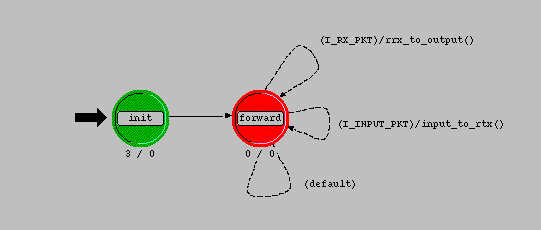
\includegraphics[width=.7\textwidth]{images/mac}
    \caption{MAC process model}
    \label{fig:appendix-d}
\end{figure}

\newpage

\section{Local variables}
\begin{figure}[ht]
    \centering
    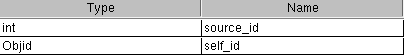
\includegraphics[width=.7\textwidth]{images/state_variable_mac}
    \caption{State variables of MAC process}
    \label{fig:appendix-d_sv}
\end{figure}

\section{Header Block}
%_____________________________________HEADER______________________________________
{\tiny
\begin{verbatim}
//Streams
#define STRM_INPUT		0
#define STRM_RRX		1
#define STRM_OUTPUT 	0
#define STRM_RTX		1
//Interrupts
#define I_RX_PKT		(op_intrpt_type() == OPC_INTRPT_STRM && op_intrpt_strm() == STRM_RRX)
#define I_INPUT_PKT		(op_intrpt_type() == OPC_INTRPT_STRM && op_intrpt_strm() == STRM_INPUT)
void rrx_to_output(void);
void input_to_rtx(void);

\end{verbatim}
}

\section{Function Block}
%______________________________FUNCTION__________________________________
{\tiny
\begin{verbatim}

void rrx_to_output(void)
{
	Packet *pPkt;
	Objid pktsource;
	char message_str[255];
	FIN(rrx_to_output());
	pPkt = op_pk_get(STRM_RRX);
	op_pk_nfd_get(pPkt, "mac_source", &pktsource);
	if(pktsource == self_id)
	{		
		op_pk_destroy(pPkt);
	}
	else
	{
		op_pk_send(pPkt, STRM_OUTPUT);
	}
	FOUT;
}
void input_to_rtx(void)
{
	Packet *pPkt;
	FIN(input_to_rtx());
	pPkt = op_pk_get(STRM_INPUT);
	op_pk_nfd_set_objid(pPkt, "mac_source", self_id);
	op_pk_send(pPkt, STRM_RTX);
	FOUT;
}

\end{verbatim}
}

\section{init State: Enter Executives}
%______________________________________Init_____________________________________________________________
{\tiny
\begin{verbatim}
self_id = op_id_self();
op_ima_obj_attr_get (self_id, "Source ID", &source_id);

\end{verbatim}
}


\cleardoublepage

%%appendix E
%HOLD QUEUE

%\section{Process: Hold Queue}

\section{Overview}
\begin{figure}[ht]
    \centering
    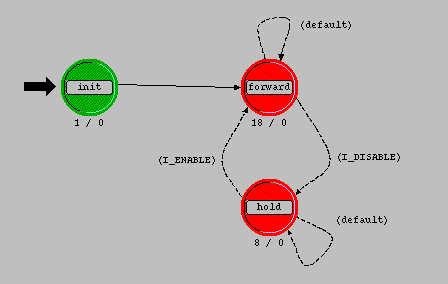
\includegraphics[width=.7\textwidth]{images/hold_queue}
    \caption{Hold queue process model}
    \label{fig:appendix-e}
\end{figure}

\newpage

\section{Local variables}
\begin{figure}[ht]
    \centering
    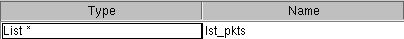
\includegraphics[width=.7\textwidth]{images/state_variable_hold_queue}
    \caption{State variables of hold queue process}
    \label{fig:appendix-e_sv}
\end{figure}

\section{Header Block}
%_____________________________________HEADER______________________________________
{\tiny
\begin{verbatim}
#define IC_DISABLE	54
#define IC_ENABLE	55
#define I_DISABLE	(op_intrpt_type() == OPC_INTRPT_REMOTE && op_intrpt_code() == IC_DISABLE)
#define I_ENABLE	(op_intrpt_type() == OPC_INTRPT_REMOTE && op_intrpt_code() == IC_ENABLE)

\end{verbatim}
}

\section{Function Block}
%______________________________FUNCTION__________________________________
{\tiny
\begin{verbatim}


\end{verbatim}
}
\section{init State: Enter Executives}
%______________________________________Init_____________________________________________________________
{\tiny
\begin{verbatim}
lst_pkts = op_prg_list_create (); 
\end{verbatim}
}

\section{forward State: Enter Executives}
%______________________________________forward_____________________________________________________________
{\tiny
\begin{verbatim}
Packet *pPkt;
int len;
len = op_prg_list_size(lst_pkts);

while(len > 0)
{
	printf("[HOLD] - Sending buffered pkt\n");
	op_pk_send(op_prg_list_remove (lst_pkts, OPC_LISTPOS_HEAD), 0);
	printf("\t[HOLD] - Done sending buffered pkt\n");
	len = op_prg_list_size(lst_pkts);	
}
pPkt = op_pk_get(0);
while(pPkt != OPC_NIL)
{
	op_pk_send(pPkt, 0);
	pPkt = op_pk_get(0);
}

\end{verbatim}
}

\section{hold State: Enter Executives}
%_____________________________________hold_____________________________________________________________
{\tiny
\begin{verbatim}
Packet *pPkt;
pPkt = op_pk_get(0);

while(pPkt != OPC_NIL)
{
	op_prg_list_insert(lst_pkts, pPkt, OPC_LISTPOS_TAIL);
	pPkt = op_pk_get(0);
}

\end{verbatim}
}

\cleardoublepage

%%appendix F
%Gateway Receiver

\section{Process: Gateway Receiver}

\subsection{Overview}
\begin{figure}[ht]
    \centering
    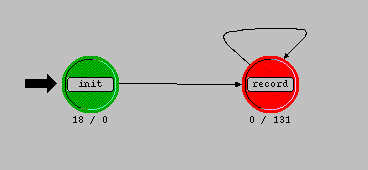
\includegraphics[width=.7\textwidth]{images/gateway_rcvr}
    \caption{Gateway receiver process model}
    \label{fig:appendix-f}
\end{figure}

% There are no local variables 

\subsection{Header Block}
%_____________________________________HEADER______________________________________
{\tiny
\begin{verbatim}
#define MAX_SRC_IDS	10
#define IC_SOURCPROP_RX 	99
int has_inited = 0;
int pkt_received[MAX_SRC_IDS*3];
int hack_pkt_keyupnum[MAX_SRC_IDS*3];
Stathandle stat_neworreplace;
Stathandle stat_counterchange;
List *create_stat_lst(char *);

\end{verbatim}
}

\subsection{Function Block}
%______________________________FUNCTION__________________________________
{\tiny
\begin{verbatim}

List *create_stat_lst(char *statName)
{
	List *lst;
	int stat_size;
	int i;
	FIN(create_stat_lst(char *statName));
	op_stat_dim_size_get (statName, OPC_STAT_GLOBAL, &stat_size);
	if(stat_size != MAX_SRC_IDS)
	{
		op_sim_end("Bad stat dimension", statName, "", "");
	}
	lst = op_prg_list_create();
	for(i = 0; i < MAX_SRC_IDS; i++)
	{
		Stathandle *sth_temp;
		sth_temp = (Stathandle *) op_prg_mem_alloc (sizeof (Stathandle));
		*sth_temp = op_stat_reg (statName, i, OPC_STAT_GLOBAL);
		op_prg_list_insert(lst, sth_temp, OPC_LISTPOS_TAIL);
	}
	FRET(lst);
}

\end{verbatim}
}
\subsection{init State: Enter Executives}
%______________________________________Init_____________________________________________________________
{\tiny
\begin{verbatim}

int stat_size_temp;
int i;
if(has_inited == 0)
{
	printf("INITIALIZING gateway statistics\n");
	has_inited = 1;
	for(i = 0; i < MAX_SRC_IDS*3; i++)
	{
		pkt_received[i] = 0;
		hack_pkt_keyupnum[i] = -1;
	}
	stat_neworreplace = op_stat_reg("Update Pkt - New or Replace" ,OPC_STAT_INDEX_NONE, OPC_STAT_GLOBAL);
	stat_counterchange = op_stat_reg("Update Counter Change" ,OPC_STAT_INDEX_NONE, OPC_STAT_GLOBAL);
}

\end{verbatim}
}

\subsection{record State: Exit Executives}
%_____________________________________Record_____________________________________________________________
{\tiny
\begin{verbatim}

Packet *pPkt;
int key;
int sourceid;
int key_updnm;
double generated_timestamp;
int is_update;
int array_index;
Objid source_prop_id;
char message_str [255];

pPkt = op_pk_get(op_intrpt_strm());
if(pPkt == OPC_NIL)
{
	op_sim_end("Nil stream pkt", "", "", "");
}
op_pk_nfd_get(pPkt, "source_id", &sourceid);
op_pk_nfd_get(pPkt, "key", &key);
op_pk_nfd_get(pPkt, "key_update_number", &key_updnm);
op_pk_nfd_get(pPkt, "source_prop_objid", &source_prop_id);
op_pk_nfd_get(pPkt, "generated_timestamp", &generated_timestamp);
//printf("\tEnd getting fields\n");

//Check the fields
if(sourceid < 0 || sourceid >= MAX_SRC_IDS)
{
	op_sim_end("Bad source id", "", "", "");
}
else if(key_updnm < 0)
{
	op_sim_end("Bad key_updnm", "", "", "");
}
else if(key < 1 || key > 3)
{
	op_sim_end("Bad key", "", "", "");
}
array_index = sourceid*3 + (key-1);
is_update = 0;
if(pkt_received[array_index])
{
	int oldkey_updnm = hack_pkt_keyupnum[array_index];
	if(oldkey_updnm < key_updnm)
	{
		is_update = 1;
		op_stat_write(stat_counterchange, key_updnm - oldkey_updnm);
		hack_pkt_keyupnum[array_index] = key_updnm;
	}
}
else
{
	is_update = 1;
	pkt_received[array_index] = 1;
	hack_pkt_keyupnum[array_index] = key_updnm;
}
if(is_update)
{
	Ici *iciptr = op_ici_create ("prop_action");
	op_ici_attr_set (iciptr, "source_id", sourceid);
	op_ici_attr_set (iciptr, "key_update_number", key_updnm);
	op_ici_attr_set (iciptr, "action", 1); //Gateway rx code
	op_ici_attr_set (iciptr, "generated_timestamp", generated_timestamp);
	op_ici_install(iciptr);
	op_intrpt_schedule_remote (op_sim_time (), IC_SOURCPROP_RX, source_prop_id);
	op_stat_write(stat_neworreplace, 1.0);
}
op_pk_destroy(pPkt);


\end{verbatim}
}


\end{appendix}
}

\ifHtml
\HCode{
<script type="text/javascript">
var gaJsHost = (("https:" == document.location.protocol) ? "https://ssl." : "http://www.");
document.write(unescape("\%3Cscript src='" + gaJsHost + "google-analytics.com/ga.js' type='text/javascript'\%3E\%3C/script\%3E"));
</script>
<script type="text/javascript">
try {
var pageTracker = _gat._getTracker("UA-12568598-3");
pageTracker._trackPageview();
} catch(err) {}</script>
}
\fi

\end{document}